\section{Auswertung}
\label{sec:Auswertung}

\subsection{Untergrund}
  Die aufgenommenen Messwerte sind in \autoref{fig:T_I_plot_beide_Messung} zu sehen.
  Der Depolarisationsstrom ist hier in Abhängigkeit von der Temperatur der Probe geplottet worden.
  Der Untergrund wird nun durch eine e-Funktion dargestellt.
  Dafür wird die Funktion
  \begin{equation*}
    f(T) = a \cdot \exp(\frac{-m}{T})
  \end{equation*}
  an den Anstieg des zweiten Maximums gefittet.
  Dabei ergeben sich folgende Werte:
  \begin{align*}
    &\text{Messung 1}\\
    &a =  \SI{4.695(2347)e9}{\pico\ampere} &&  m = \SI{5899.27(15055)}{\kelvin} \, ,\\
    &\text{Messung 2}\\
    &a = \SI{903.023(484904)e6}{\pico\ampere} &&  m = \SI{5359.79(16524)}{\kelvin} \, .\\
  \end{align*}
  In \autoref{fig:T_I_plot_Untergrund} sind die entsprechenden Untergrund-Fits zu sehen.

  \begin{figure}[H]
    \centering
    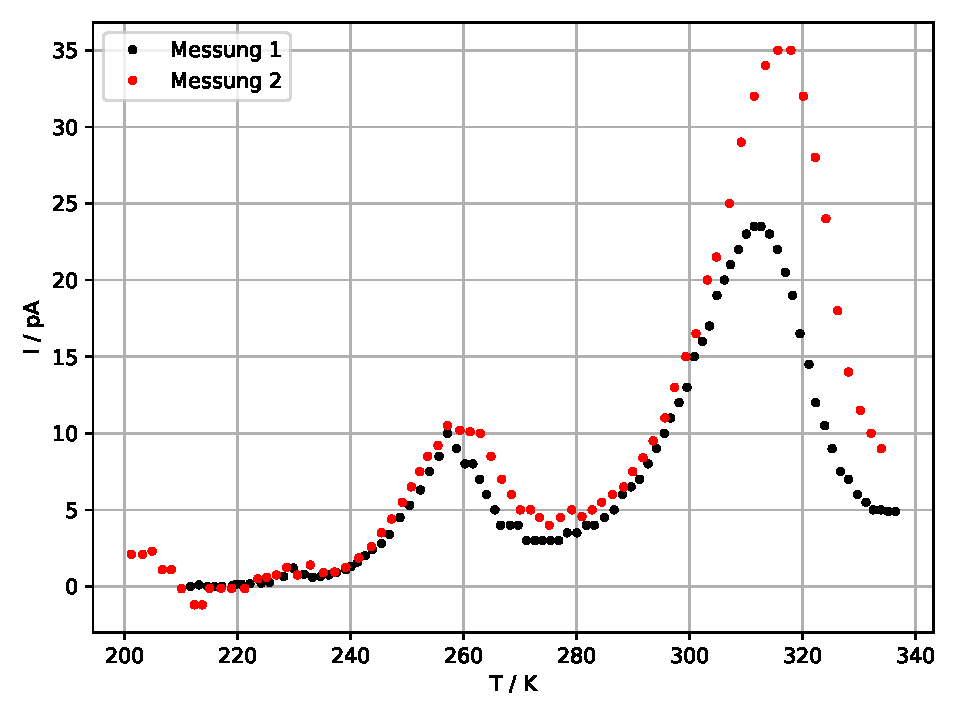
\includegraphics[width = 0.7\textwidth]{build/plot.pdf}
    \caption{Die aufgenommenen Messwerte. Bei Messung 1 wird eine Heizrate von $b = \SI{1.5}{\celsius\per\minute}$ erzielt, 
    bei Messung 2 soll $b = \SI{2}{\celsius\per\minute}$ betragen.}
    \label{fig:T_I_plot_beide_Messung}
  \end{figure} % OK

  \begin{figure}[H]
    \begin{subfigure}[b]{.5\linewidth}
      \centering
      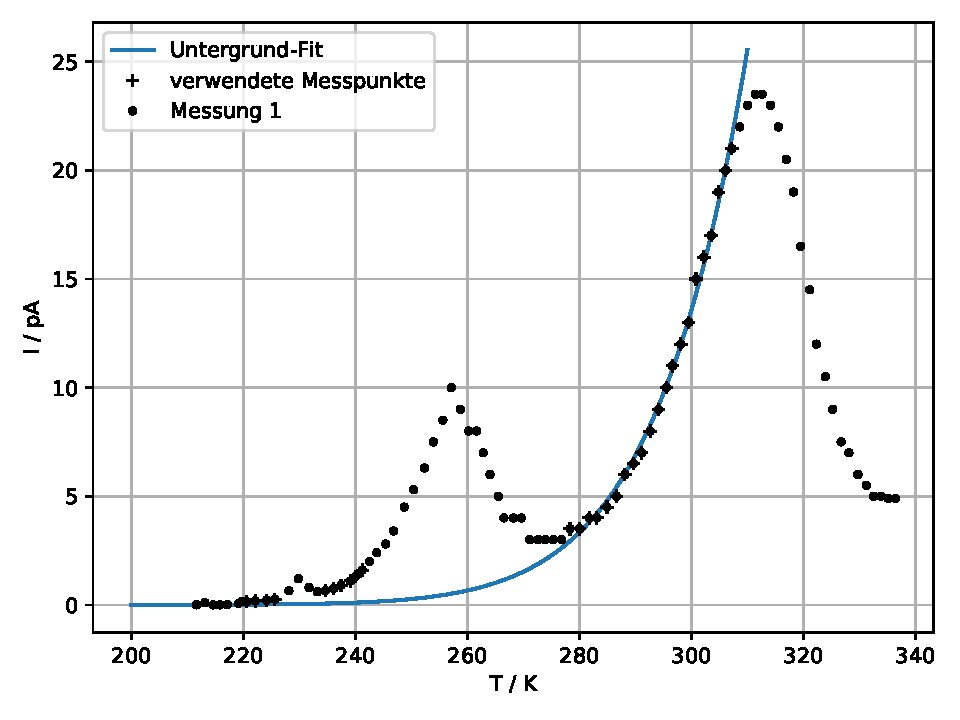
\includegraphics[height=5cm, keepaspectratio]{build/untergrund_1.pdf}
    \end{subfigure}
    \begin{subfigure}[b]{.5\linewidth}
      \centering
      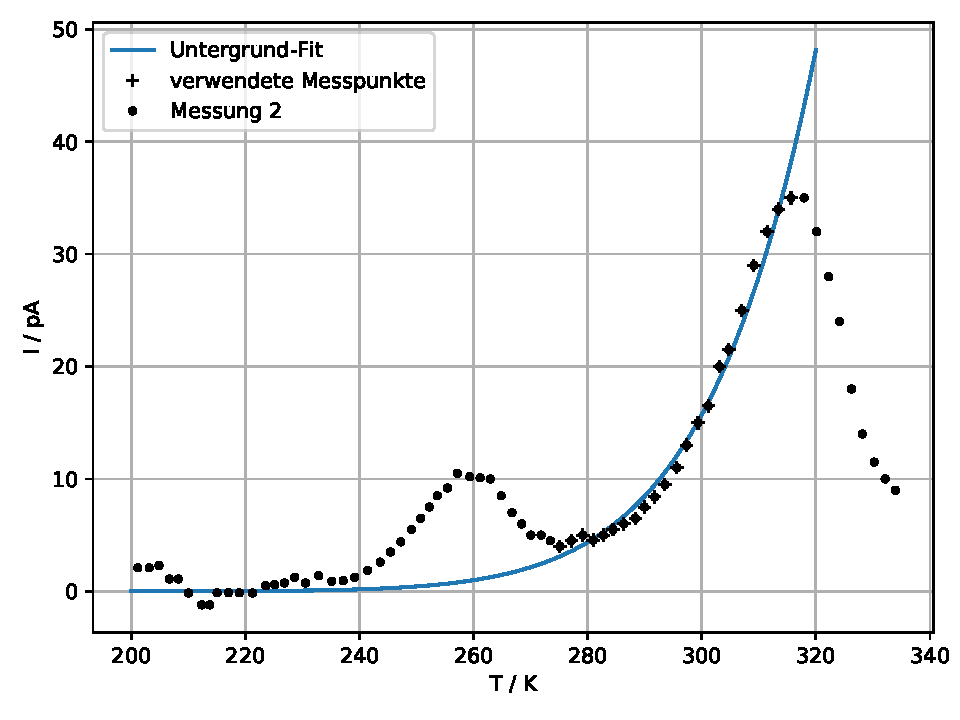
\includegraphics[height=5cm, keepaspectratio]{build/untergrund_2.pdf}
    \end{subfigure}
    
    \caption{Die gefittete Untergrundfunktion mit der Form einer e-Funktion.
      Die Messwerte, die den Anstieg des zweiten Maximums bilden, werden für den Fit verwendet.}
    \label{fig:T_I_plot_Untergrund}
  \end{figure} % OK

\subsection{Heizrate}
  Die aufgenommenen Messwerte können auch in ein Zeit-Temperatur Diagramm dargestellt werden.
  Dieses ist in \autoref{fig:t_T_plot} zu sehen.
  Um die Heizrate der jeweiligen Messung zu bestimmen, wird eine lineare Ausgleichsrechnung durhgeführt.
  Die zu fittende Funktion hat die Form
  \begin{equation*}
    T(t) = b \cdot t + T_0 \, .
  \end{equation*}
  Es ergibt sich für die erste Messung:
  \begin{align*}
    b = \SI{14.6(04)e-1}{\kelvin\per\minute} &&  T_0 = \SI{210.92(19)}{\kelvin}\\
  \end{align*}
  und für die zweite Messung:
  \begin{align*}
    b =  \SI{18.7(05)e-1}{\kelvin\per\minute}  &&  T_0 = \SI{198.95(20)}{\kelvin} \, . \\
  \end{align*}
  Die beiden Messungen sowie ihre jeweiligen Ausgleichsgeraden sind in \autoref{fig:t_T_plot_1_Ausgleich} und \autoref{fig:t_T_plot_2_Ausgleich} zu sehen.

  \begin{figure}[H]
    \centering
    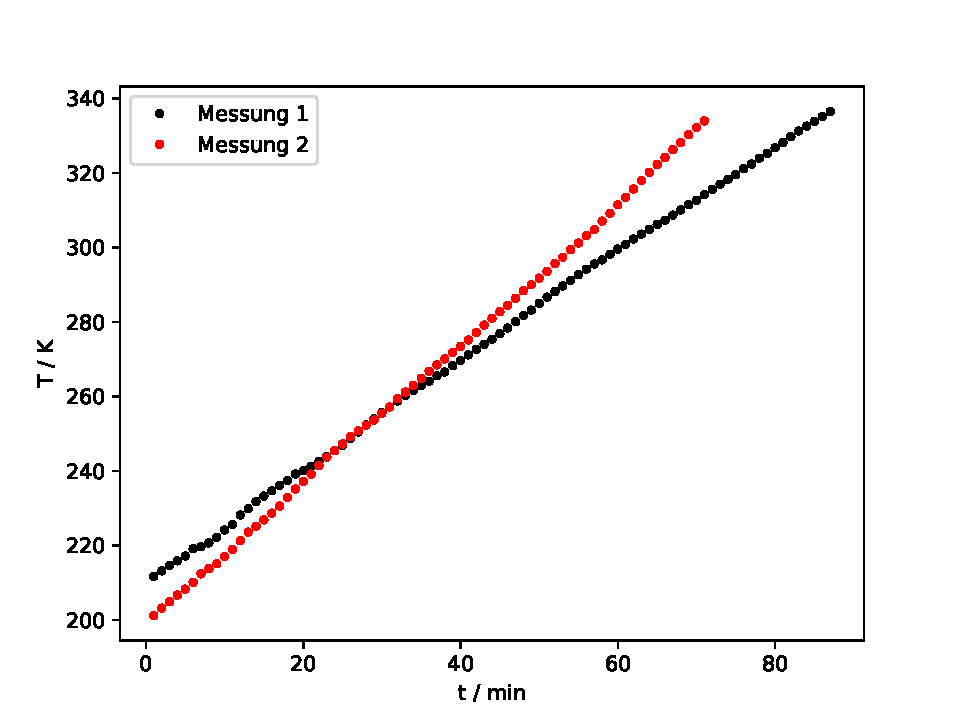
\includegraphics[width = 0.7\textwidth]{build/zeit_temp.pdf}
    \caption{Die aufgenommenen Messwerte. Bei Messung 1 wird eine Heizrate von $b = \SI{1.5}{\kelvin\per\minute}$ erzielt, 
    bei Messung 2 soll $b = \SI{2}{\kelvin\per\minute}$ betragen.}
    \label{fig:t_T_plot}
  \end{figure} % OK, eig könnte man beschreibung so lassen bzw. wat soll man sonst da schreiben

  \begin{figure}[H]
    \begin{subfigure}[b]{.5\linewidth}
      \centering
      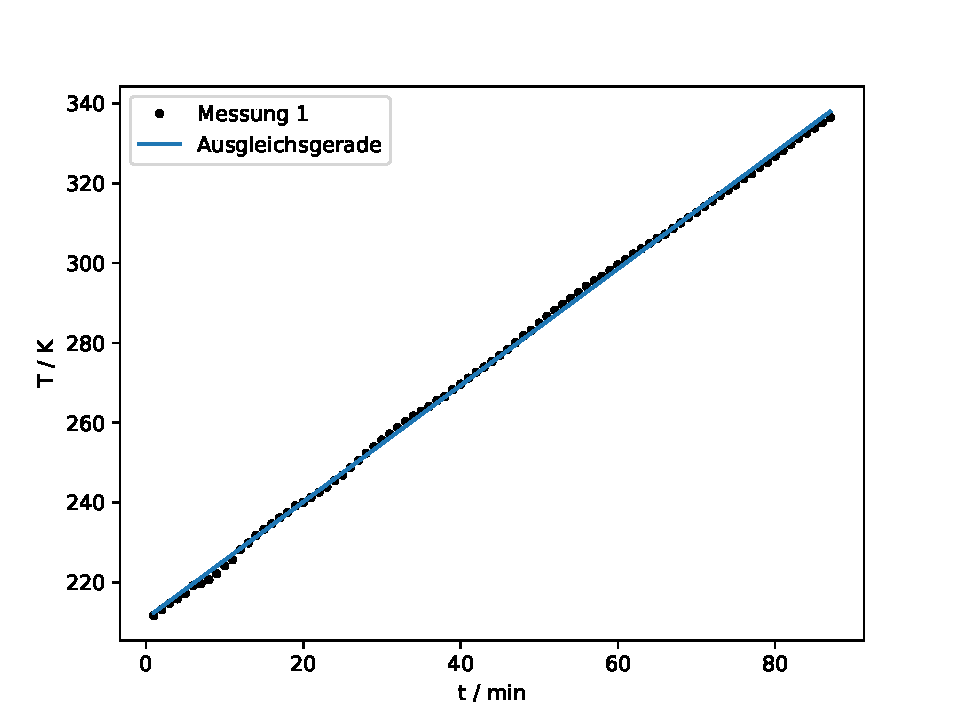
\includegraphics[height=5cm, keepaspectratio]{build/zeit_temp_fit_1.pdf}
      \caption{Durch den Fit ergibt sich für $\SI{1.46(0037)}{\kelvin\per\minute}$.}
    \label{fig:t_T_plot_1_Ausgleich}
    \end{subfigure}
    \begin{subfigure}[b]{.5\linewidth}
      \centering
      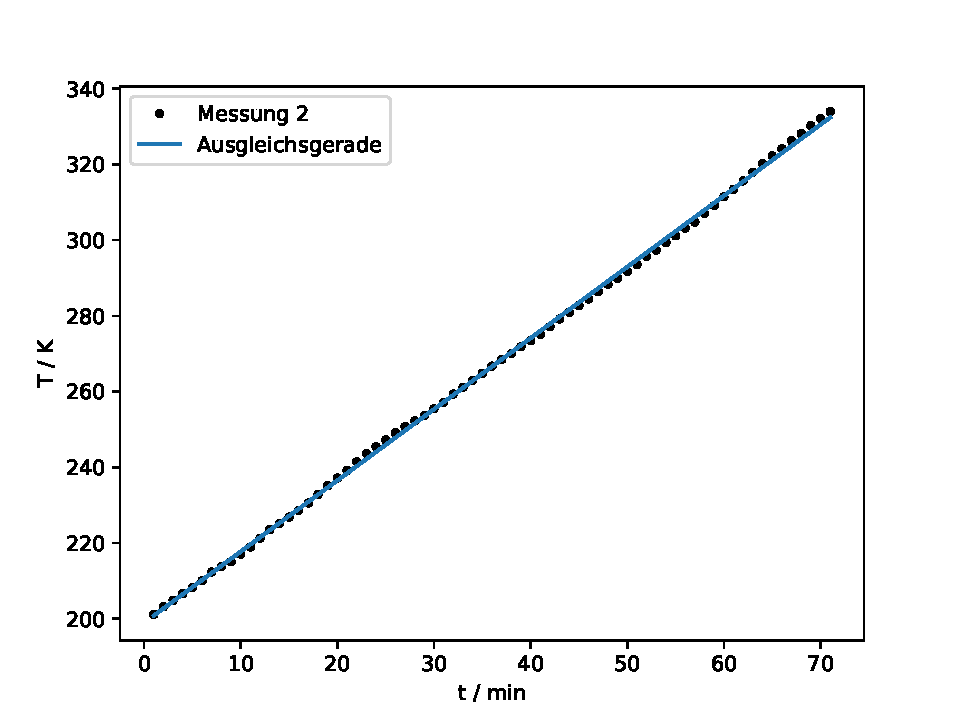
\includegraphics[height=5cm, keepaspectratio]{build/zeit_temp_fit_2.pdf}
      \caption{Durch den Fit ergibt sich für $b = \SI{1.87(0049)}{\kelvin\per\minute}$.}
    \label{fig:t_T_plot_2_Ausgleich} 
    \end{subfigure}
    \caption{Die aufgenommenen Messwerte der Messungen und der dazugehörige Fit um die Heizrate zu bestimmen.}
  \end{figure} % OK

\subsection{Aktivierungsenergie - Erste Methode}
  Zur Bestimmung der Aktivierungsenergie mithilfe des Maximums werden die Messwerte zunächst in eine andere Darstellung gebracht.
  Nach \eqref{eqn:geradengleichung} wird der Logarithmus des Depolarisationsstrom gebildet und gegen die inverse Temperatur abgebildet.
  Die jeweiligen Diagramme sind in \autoref{fig:log_I_1_durch_T_Messung_1} und \autoref{fig:log_I_1_durch_T_Messung 2} zu finden.
  Mithilfe von python wird eine Ausgleichsrechnung durchgeführt.
  Die zu fittende Funktion hat dabei die Form
  \begin{equation*}
    \ln{I(T)} = c - m \cdot \frac{1}{T} \, .
  \end{equation*}
  Die ermittelten Werte sind für Messung 1:
  \begin{align*}
    c =  \SI{31.97(62)}{\ln(\pico\ampere)} && m = (-7618,67\pm 150,70)\,\si{\kelvin} \,  \\
  \end{align*}
  und für Messung 2:
  \begin{align*}
    c = \SI{22.90(184)}{\ln(\pico\ampere)} && m = (-5348,16\pm 444,14)\,\si{\kelvin}  \, . \\
  \end{align*}
  Die Ausgleichsgeraden sind ebenfalls in \autoref{fig:log_I_1_durch_T_Messung_1} und \autoref{fig:log_I_1_durch_T_Messung 2} zu finden.

  \begin{figure}[H]
    \begin{subfigure}[b]{.5\linewidth}
      \centering
      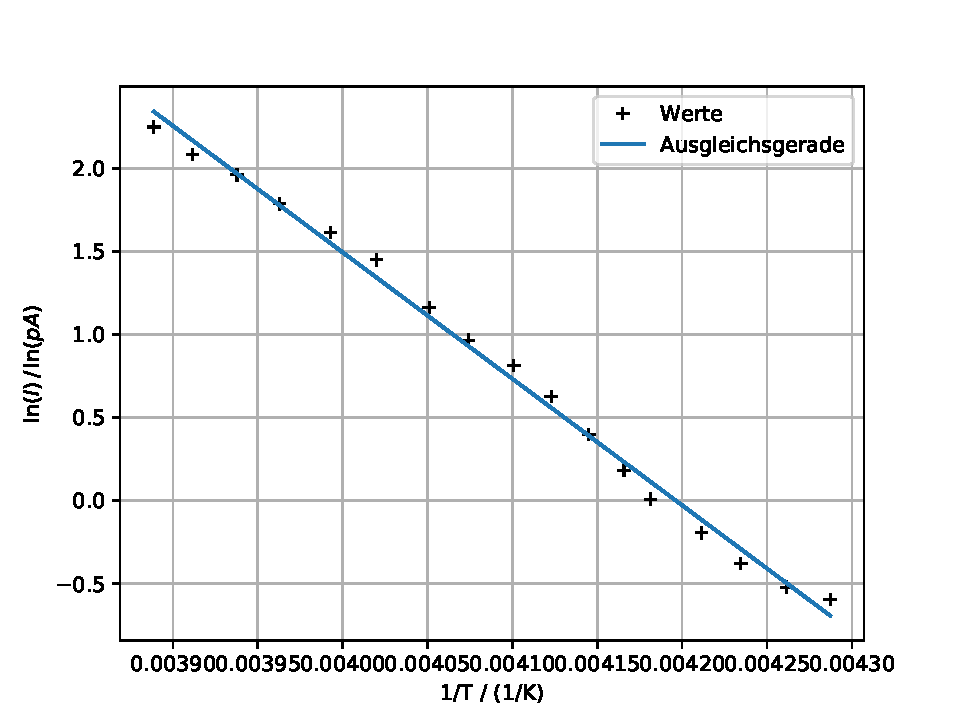
\includegraphics[height=5cm, keepaspectratio]{build/log(I)_1durchT_1.pdf}
      \caption{Die verwendeten Messwerte aus der Messung 1.}
      \label{fig:log_I_1_durch_T_Messung_1}
    \end{subfigure}
    \begin{subfigure}[b]{.5\linewidth}
      \centering
      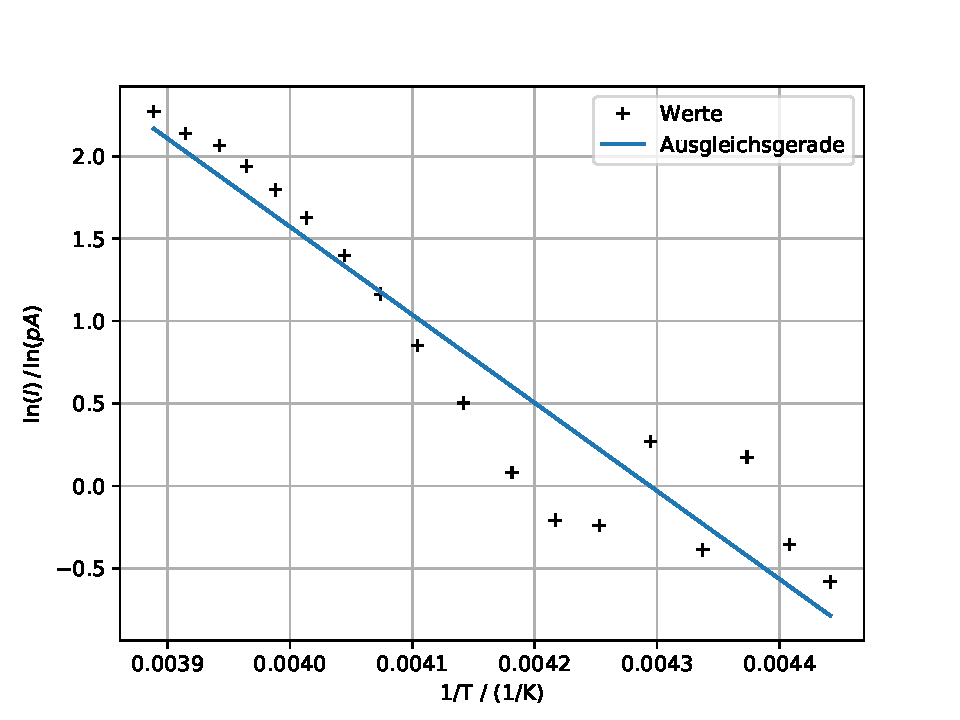
\includegraphics[height=5cm, keepaspectratio]{build/log(I)_1durchT_2.pdf}
      \caption{Die verwendeten Messwerte aus der Messung 2}
      \label{fig:log_I_1_durch_T_Messung 2}
    \end{subfigure}
    \caption{Die korrigierten Messwerte. Nur der erste Peak wurde betrachtet. Durch die veränderte Darstellungsweise wird eine Ausgleichsrechnung durchgeführt.}
  \end{figure} % Ok

  \noindent
  Aus \eqref{eqn:Aktivierungsenergie} ergibt sich dann für die jeweilige Aktivierungsenergie $W$
  \begin{align*}
    W   &= -k_\text{B} \cdot m \\
    \implies W_{1,1} &= \SI{1.052(021)e-19}{\joule} &= \SI{0.657(013)}{\electronvolt} \, , \\
    \implies W_{1,2} &= \SI{7.4(6)e-20}{\joule} &= \SI{0.460(40)}{\electronvolt}  \, .\\
  \end{align*}

\subsection{Aktivierungsenergie - Zweite Methode}
  Der korrigierte Stromverlauf wird nun betrachtet.
  Dieser ist für beide Messungen in \autoref{fig:I_T_korrigiert} zu finden.

  \begin{figure}[H]
    \begin{subfigure}[b]{.5\linewidth}
      \centering
      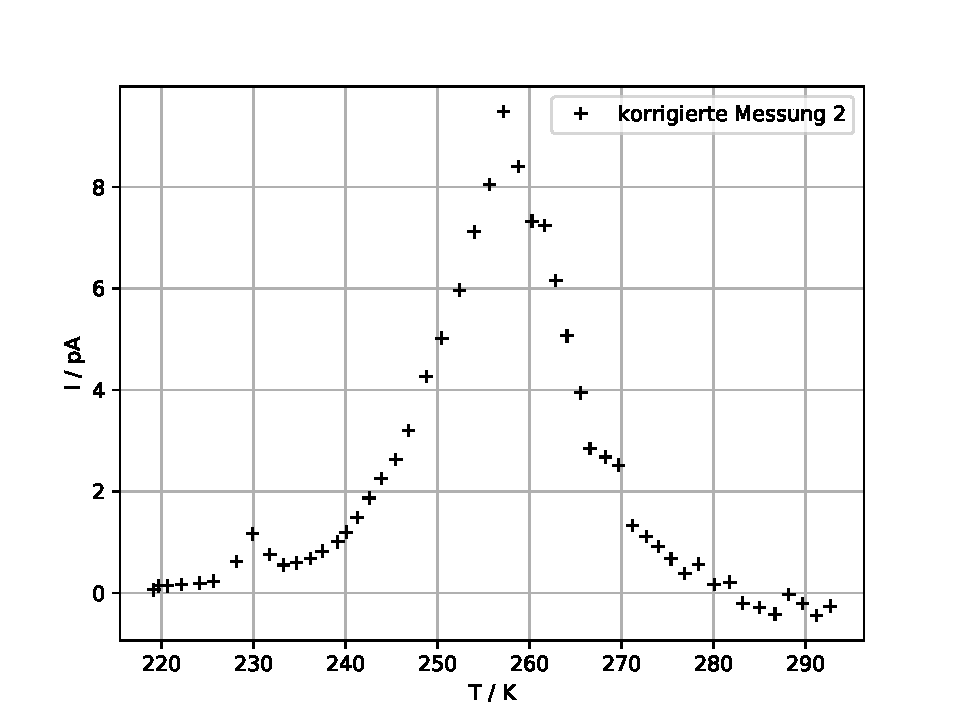
\includegraphics[height=5cm, keepaspectratio]{build/korrigierte_werte_1.pdf}
    \end{subfigure}
    \begin{subfigure}[b]{.5\linewidth}
      \centering
      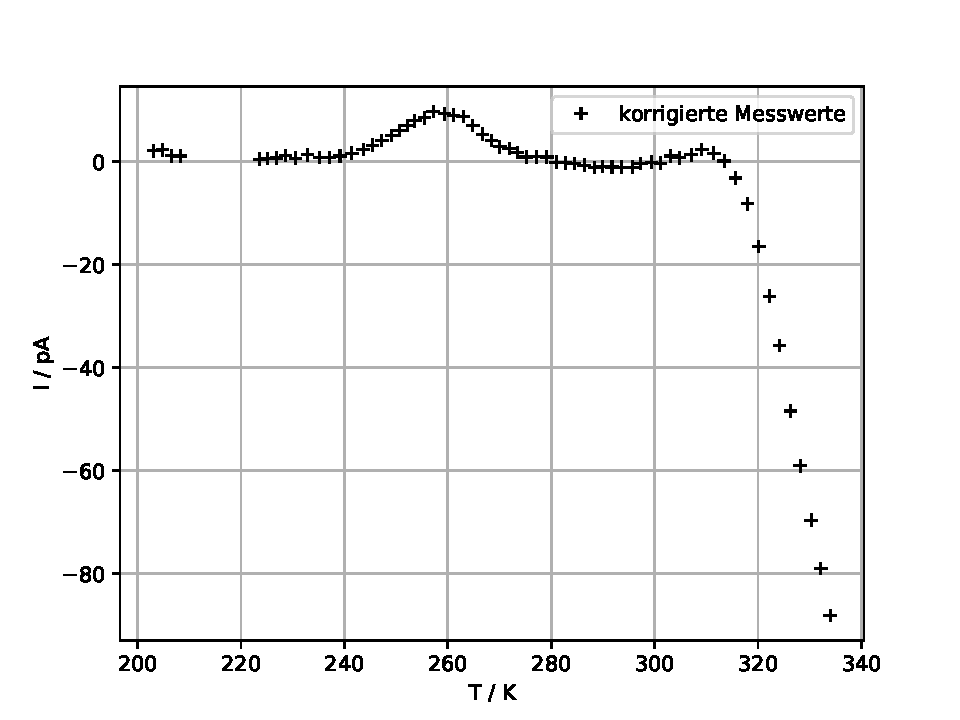
\includegraphics[height=5cm, keepaspectratio]{build/korrigierte_werte_2.pdf}
    \end{subfigure}
    \caption{Die Messwerte der jeweiligen Messung nach Abzug des Untergrunds.}
    \label{fig:I_T_korrigiert}
  \end{figure} % OK idk

  \noindent
  Zusätzlich wird nur der Peak der jeweiligen Messung betrachtet.
  Nach \eqref{eqn:fur_Integral} wird $\frac{1}{T}$ gegen $\ln\left( \frac{\int_T^\infty I(T') \, \text{d}T'}{b \tau_0 \cdot I(T)}\right)$ aufgenommen um dadurch eine lineare Ausgleichsrechnung der Form
  \begin{equation*}
    y = m \cdot x + b 
  \end{equation*}
  durchzuführen.
  Dazu wird das Integral, das im Logarithmus steht mithilfe von python bestimmt.
  Die Diagramme mit den dazugehörigen Ausgleichsgeraden sind in \autoref{fig:Trapez} zu finden.
  Die ermittelten Werte betragen:
  \begin{align*}
    &\text{Messung 1} \\
    &m = (9541.25 \pm 135.01)\,\si{\kelvin} && b= -34.97 \pm  \, 0.54 , \\ 
    &\text{Messung 2} \\
    &m = (10269.27 \pm 133.28)\,\si{\kelvin} && b = -37.83 \pm 0.53\, . \\
  \end{align*}
  \noindent
  Mithilfe von \eqref{eqn:Aktivierungsenergie} wird die Aktivierungsenergie $W$ bestimmt.
  Es folgt:
  \begin{align*}
    W_{2,1} &= \SI{1.317(019)e-19}{\joule} &= \SI{0.822(012)}{\electronvolt} \, ,\\
    W_{2,2} &= \SI{1.418(018)e-19}{\joule} &= \SI{0.885(011)}{\electronvolt} \, .\\
  \end{align*}

  \begin{figure}[H]
    \begin{subfigure}[b]{.5\linewidth}
      \centering
      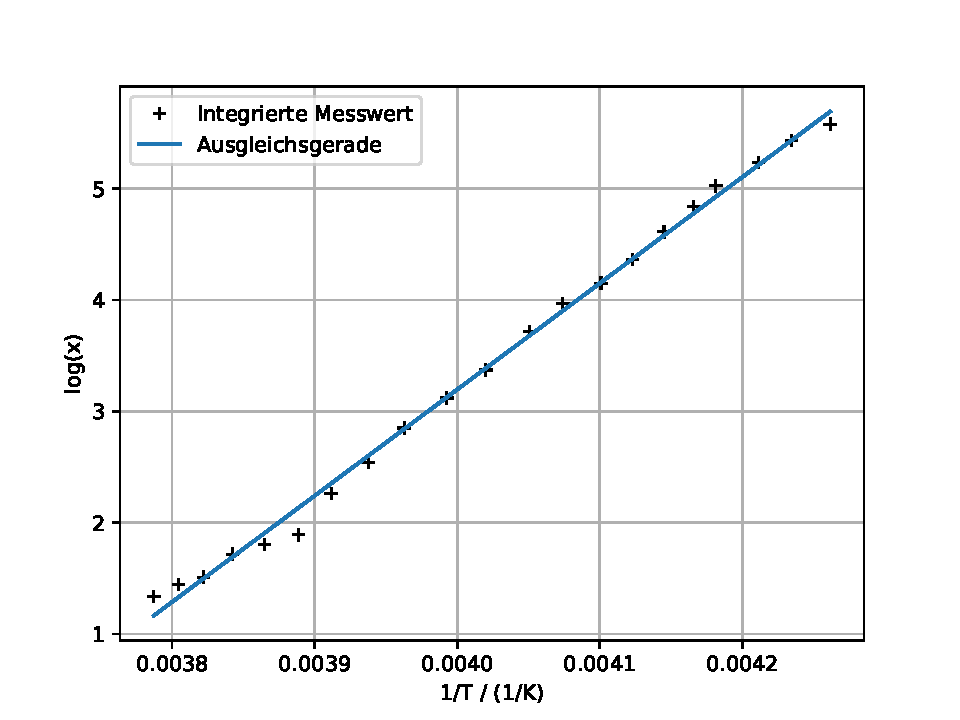
\includegraphics[height=5cm, keepaspectratio]{build/log(int)_2durchT_1.pdf}
      \caption{Messung 1}
    \end{subfigure}
    \begin{subfigure}[b]{.5\linewidth}
      \centering
      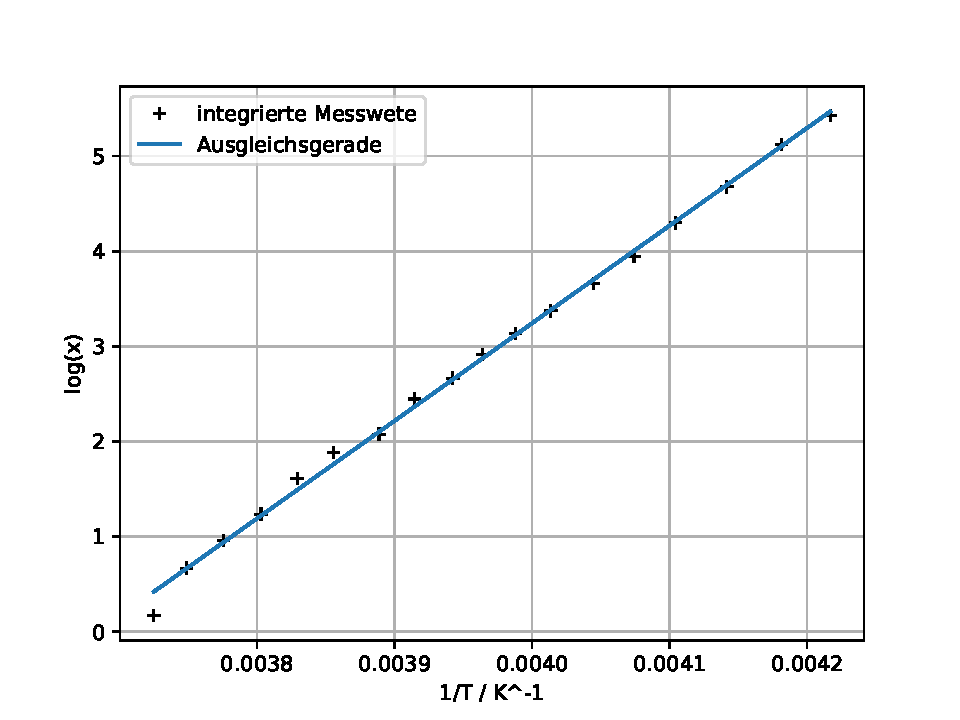
\includegraphics[height=5cm, keepaspectratio]{build/log(int)_2durchT_2.pdf}
      \caption{Messung 2}
    \end{subfigure}
    \caption{Die nach der Vorschrift integrierten Messwerte und die jeweiligen Ausgleichsgeraden zur Bestimmung der Aktivierungsenergie nach der zweiten Methode.
      Hierbei definiert $x = \frac{\int_T^\infty I(T') \, \text{d}T'}{b \tau_0 \cdot I(T)}$}
    \label{fig:Trapez}
  \end{figure} % OK Beschreibbung

\subsection{Relaxationszeit}
  Mit den ermittelten Heizraten und Aktivierungsenergien kann nach \eqref{eqn:auswertungrelax} die Relaxationszeit bestimmt werden.
  Die Heizrate für Messung 1 beträgt $b_1 = \SI{14.6(04)e-1}{\kelvin\per\minute}$ und für Messung 2 $b_2 = \SI{18.7(05)e-1}{\kelvin\per\minute}$.
  Somit folgt für die jeweilige Relaxationszeit $\tau$ mit den Aktivierungsenergien $W$ aus der ersten Methode:
  \begin{align*}
    \tau_{1,1} = (4\pm 6)\cdot 10^{-7}\,\si{\minute} &&  \tau_{1,2} = (2,1\pm 1)\cdot 10^{-10}\,\si{\minute} \, . \\
  \end{align*}
  Dabei wurde für $T_\text{max,1} = \SI{38.3}{\celsius} = \SI{311.45}{\kelvin} $ und $T_\text{max,2} = \SI{42.5}{\celsius} = \SI{315.65}{\kelvin}$ ermittelt.
  Bei dieser Temperatur wurde der maximale Depolarisationsstrom beobachtet.

  \noindent
  Mithilfe der zweiten Methode wird die Relaxationszeit auch mit \eqref{eqn:auswertungrelax} bestimmt.
  Es folgt für die jeweilige Messung:
  \begin{align*}
    \tau_{2,1} =  (3,5\pm 1,5)\cdot 10^{-13}\,\si{\minute} &&  \tau_{2,2} = (3,8\pm 1,7)\cdot 10^{-14}\,\si{\minute}\, . \\
  \end{align*}
